% !TEX root =  ../report.tex
\section{Introduction}

This paper consists of an evaluation of the prototype of the Talio application for Object Oriented Programming Project (OOPP). The objective of this evaluation is to reflect on usability problems encountered by five reviewers and from these create solutions which will improve the overall usability of the application. 

The prototype was developed by the authors of this paper using the online tool Moqups. It shows the general appearance of the User Interface using geometric shapes, images and text.

\begin{figure}[h]
    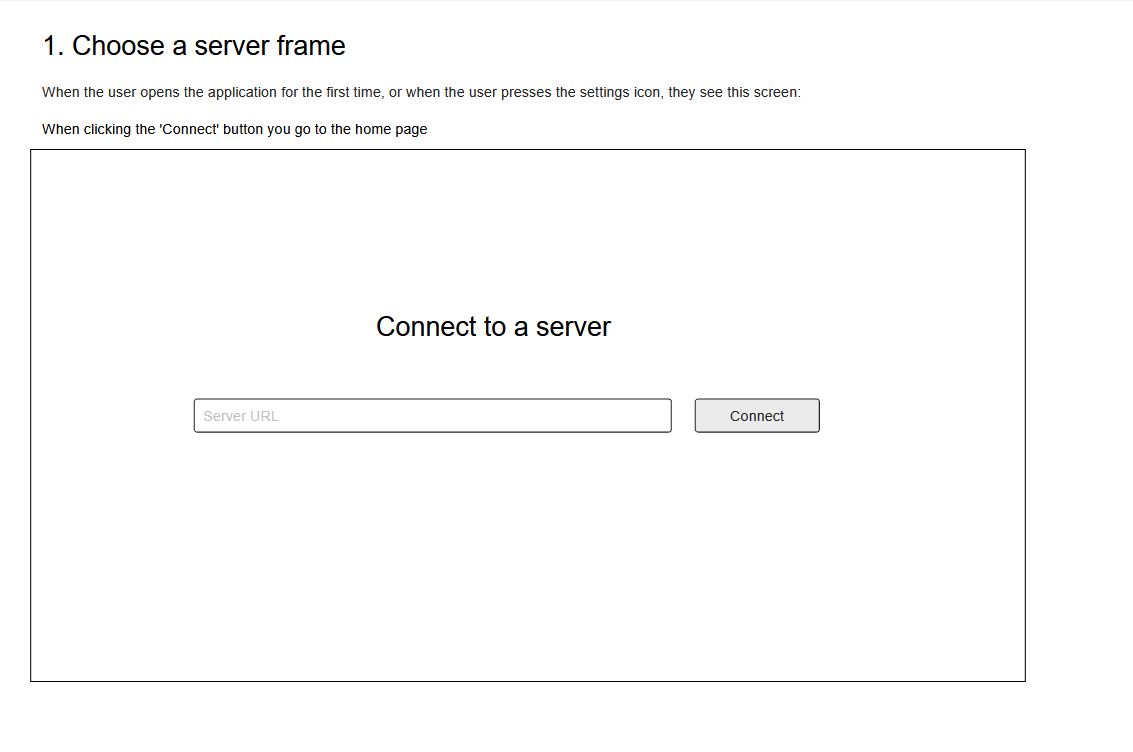
\includegraphics[width=0.4\textwidth]{content/images/1.ServerFrame.png}
    \caption{The server frame}
    \label{fig:server-frame}
\end{figure}

\begin{figure}[h]
    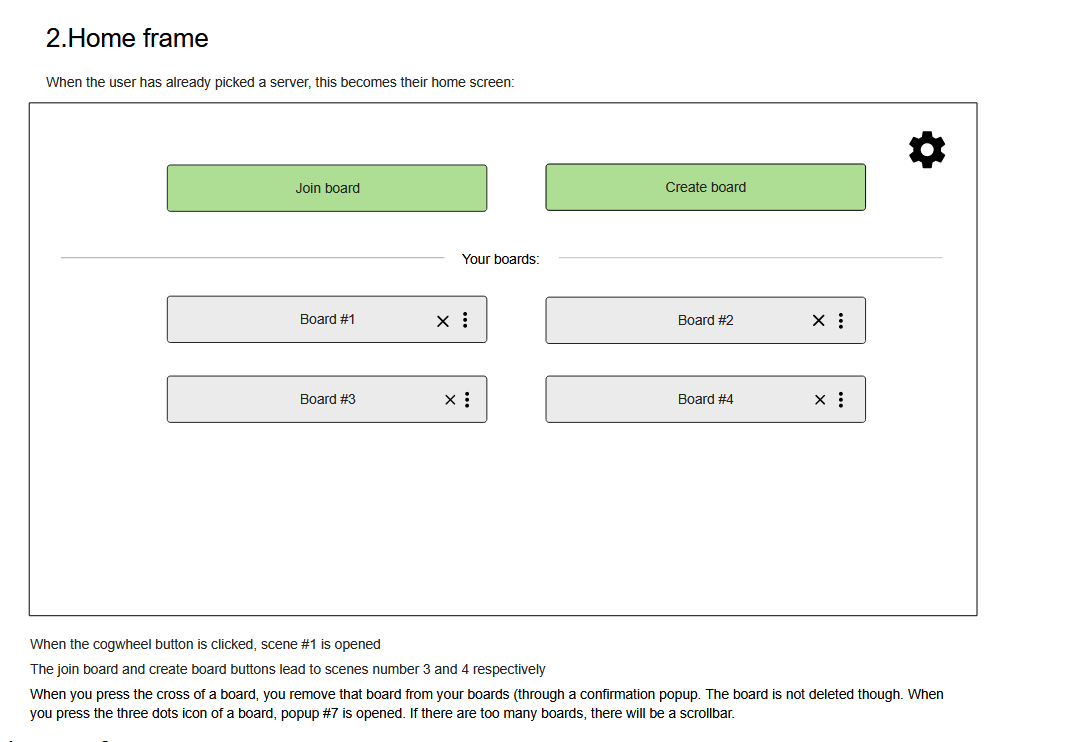
\includegraphics[width=0.4\textwidth]{content/images/2.HomeFrame.png}
    \caption{The home frame}
    \label{fig:home-frame}
\end{figure}

\begin{figure}[h]
    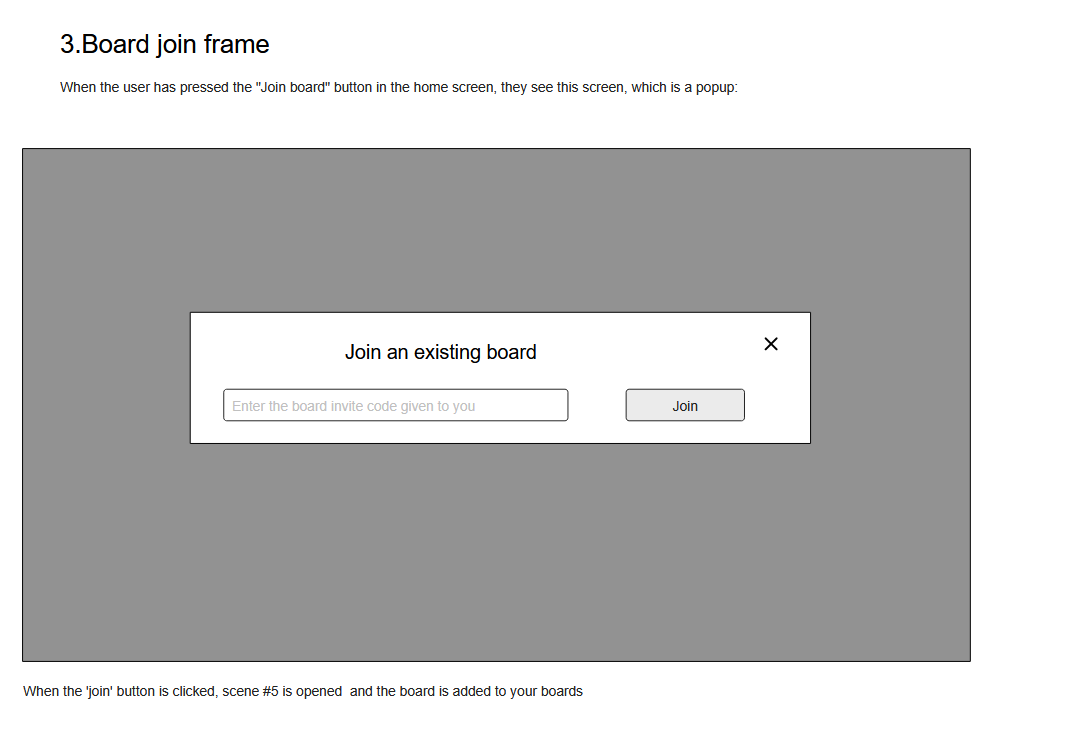
\includegraphics[width=0.4\textwidth]{content/images/3.BoardJoin.png}
    \caption{The join board frame}
    \label{fig:board-join}
\end{figure}

\begin{figure}[h]
    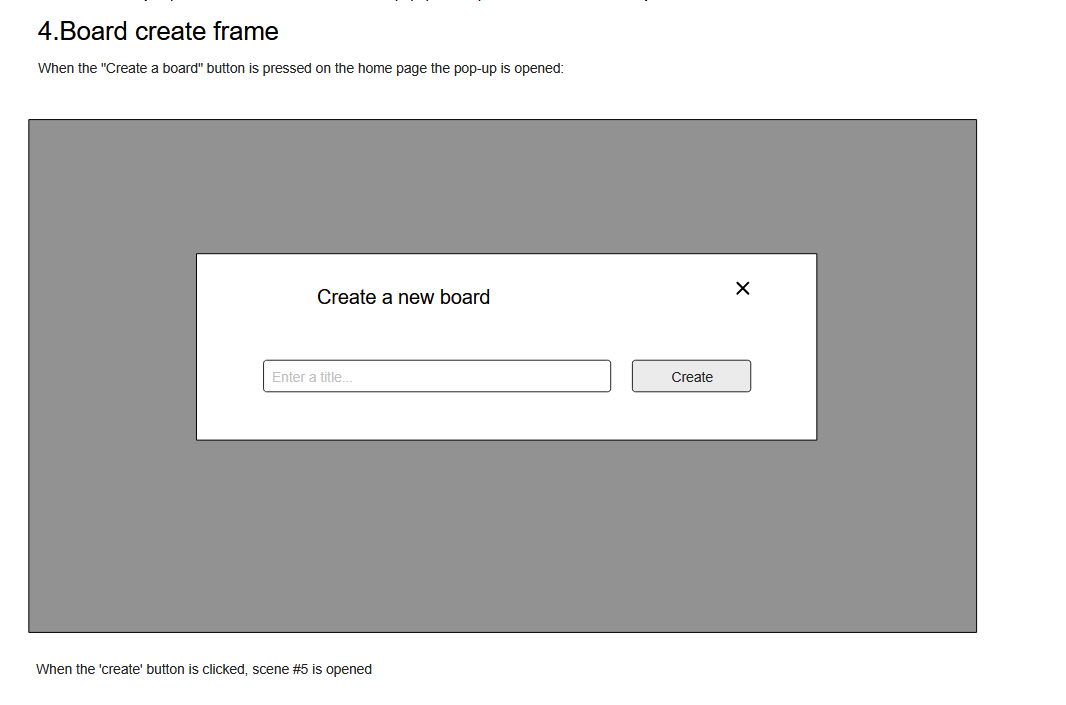
\includegraphics[width=0.4\textwidth]{content/images/4.BoardCreate.png}
    \caption{The create board frame}
    \label{fig:board-create}
\end{figure}

\begin{figure}[h]
    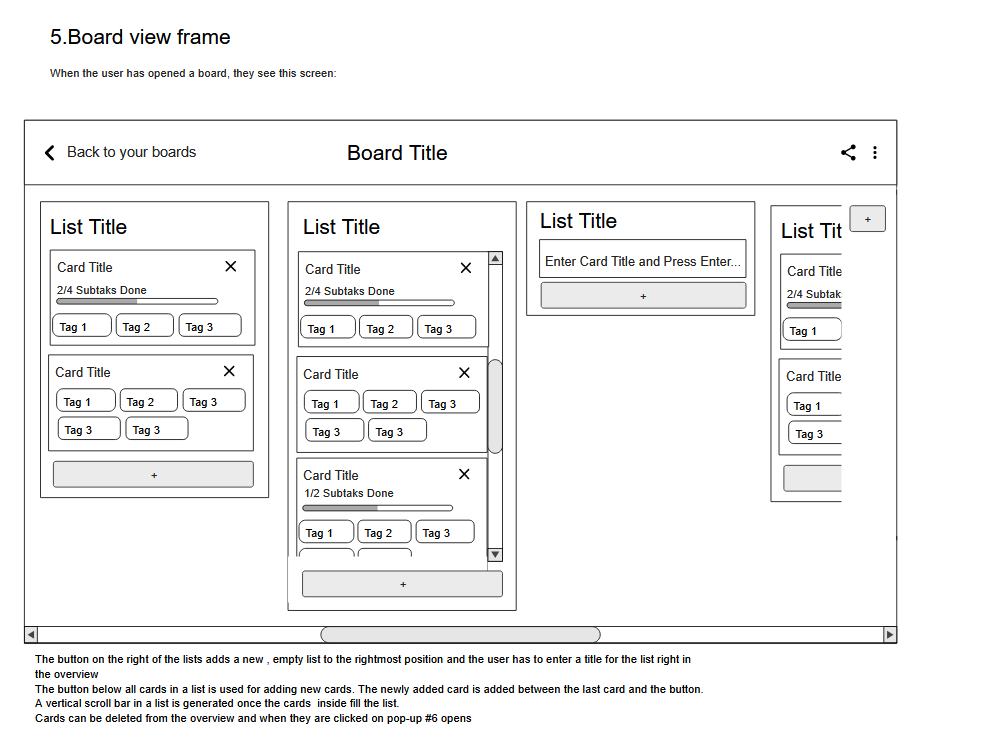
\includegraphics[width=0.4\textwidth]{content/images/5.BoardView.png}
    \caption{The view board frame}
    \label{fig:board-view}
\end{figure}

\begin{figure}[h]
    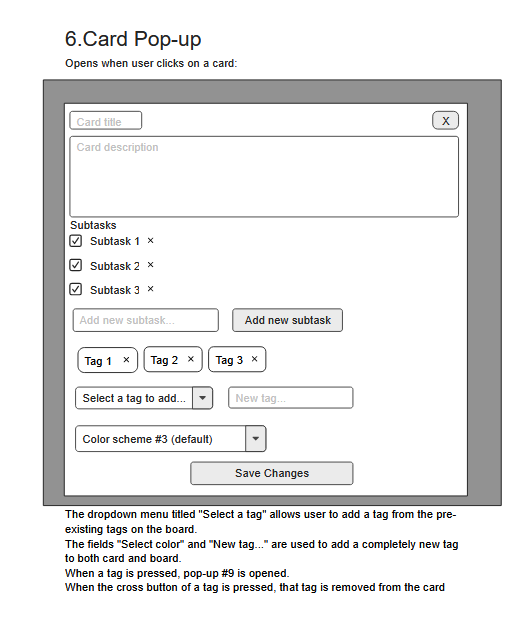
\includegraphics[width=0.4\textwidth]{content/images/6.CardPopup.png}
    \caption{The card popup frame}
    \label{fig:card-popup}
\end{figure}

\begin{figure}[h]
    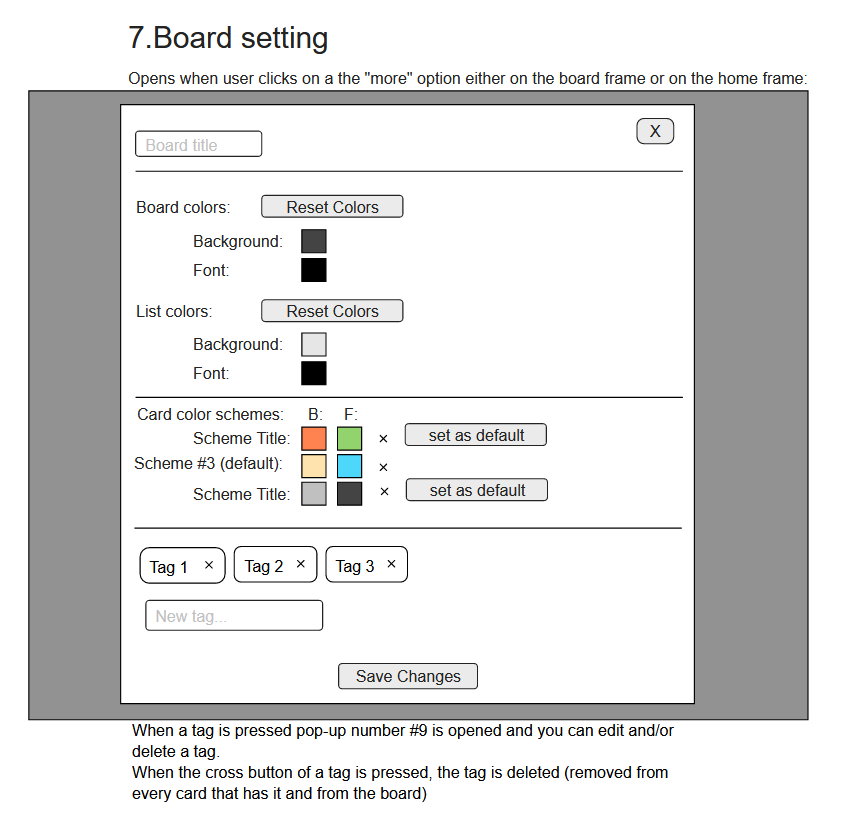
\includegraphics[width=0.4\textwidth]{content/images/7.BoardSetting.png}
    \caption{The board settings frame}
    \label{fig:board-settings}
\end{figure}

\begin{figure}[h]
    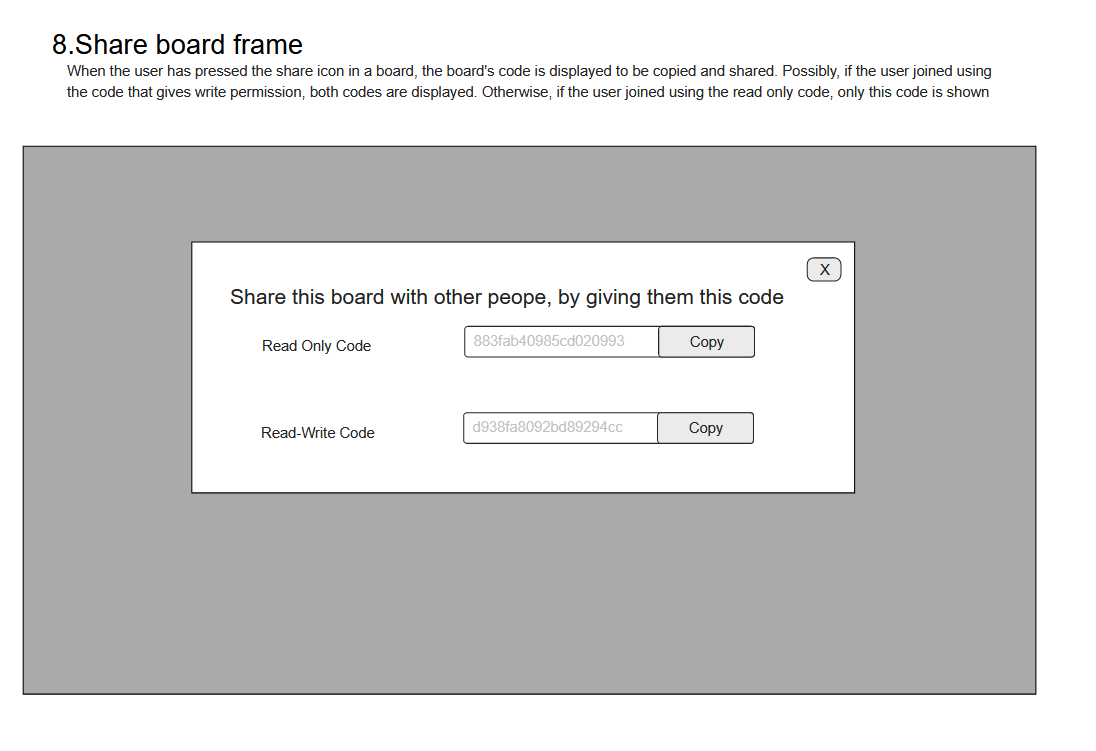
\includegraphics[width=0.4\textwidth]{content/images/8.ShareBoard.png}
    \caption{The share board frame}
    \label{fig:board-share}
\end{figure}

\begin{figure}[h]
    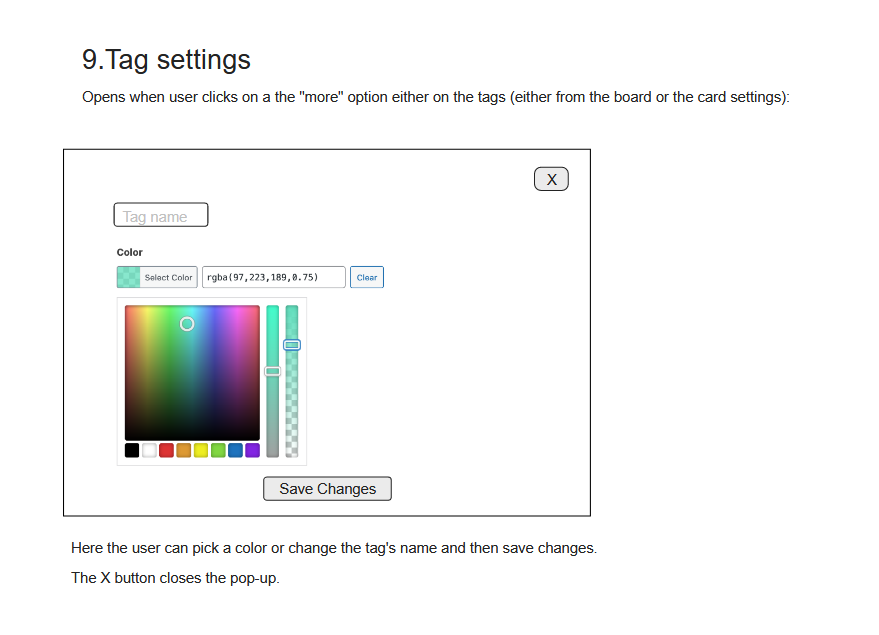
\includegraphics[width=0.4\textwidth]{content/images/9.TagSettings.png}
    \caption{The tag settings frame}
    \label{fig:tag-settings}
\end{figure}

\newpage











